%%%%%%%%%%%%%%%%%%%%%%%%%%%%%%%%%%%%%%%%%%%%%%%%%%%%%%%%%%%%%%%%%%%%%%%%%%%%%%%%
% CS 2640 Final Project Paper
%%%%%%%%%%%%%%%%%%%%%%%%%%%%%%%%%%%%%%%%%%%%%%%%%%%%%%%%%%%%%%%%%%%%%%%%%%%%%%%%

\documentclass[letterpaper,twocolumn,10pt]{article}
\usepackage{usenix-2020-09}
\usepackage{tikz}
\usetikzlibrary{shapes.geometric, arrows, positioning, fit, calc}
\usepackage{amsmath}
\usepackage{booktabs}
\usepackage{graphicx}
\usepackage{hyperref}

% inlined bib file
\usepackage{filecontents}

%-------------------------------------------------------------------------------
\begin{filecontents}{\jobname.bib}
%-------------------------------------------------------------------------------
@inproceedings{qin2025mooncake,
  title={Mooncake: Trading More Storage for Less Computation — A KVCache-centric Architecture for Serving LLM Chatbot},
  author={Qin, Ruoyu and others},
  booktitle={USENIX FAST '25},
  year={2025}
}
@misc{allison2025towards,
  title={Towards Efficient Flash Caches with Emerging NVMe Flexible Data Placement SSDs},
  author={Allison and others},
  howpublished={EuroSys '25 / arXiv:2503.11665},
  year={2025}
}
@inproceedings{hao2026fast,
  title={Fast Cloud Storage for AI Jobs via Grouped I/O API with Transparent Read/Write Optimizations},
  author={Hao and others},
  booktitle={USENIX FAST '26},
  year={2026}
}
@misc{purandare2025valet,
  title={Valet: Efficient Data Placement on Modern SSDs},
  author={Purandare, Devashish R. and others},
  howpublished={SoCC '25 / arXiv:2501.00977},
  year={2025}
}
@article{park2025fdpvirt,
  title={FDPVirt+: Emulated Flexible Data Placement for Sustainable SSDs},
  author={Park, Joonyeop and Eom, Hyeonsang},
  journal={IEEE Access},
  year={2025}
}
@inproceedings{bjorling2021zns,
  title={ZNS: Avoiding the Block Interface Tax for Flash-based SSDs},
  author={Bj{\o}rling, Matias and others},
  booktitle={USENIX ATC '21},
  year={2021}
}
@inproceedings{cooper2010ycsb,
  title={Benchmarking cloud serving systems with YCSB},
  author={Cooper, Brian F. and others},
  booktitle={Proceedings of the 1st ACM symposium on Cloud computing},
  year={2010}
}
@inproceedings{berg2020cachelib,
  title={The CacheLib Caching Engine: Design and Experiences at Scale},
  author={Berg, Benjamin and others},
  booktitle={USENIX OSDI '20},
  year={2020}
}
\end{filecontents}

%-------------------------------------------------------------------------------
\begin{document}
%-------------------------------------------------------------------------------

\date{}

\title{\Large \bf Bridging the Semantic Gap: An Evaluation of ZNS and FDP in Cloud Environments}

\author{
{\rm Howard Huang}\\
CS2640 Final Project
}

\maketitle

%-------------------------------------------------------------------------------
\begin{abstract}
%-------------------------------------------------------------------------------
Modern Solid State Drives (SSDs) inherently suffer from a ``semantic gap'' where internal device controllers remain oblivious to application-level data lifetimes. This disconnect induces a ``log-on-log'' problem, triggering redundant garbage collection at both the host filesystem and device flash translation layers. The result is inflated Write Amplification Factors (WAF) and latency spikes. Recent architectural extensions to the NVMe protocol—specifically Zoned Namespaces (ZNS) and Flexible Data Placement (FDP)—offer mechanisms to align host software with flash geometries. However, empirical comparisons of ZNS's strict host-managed zones against FDP's hint-based heuristics are scarce due to hardware unavailability. This paper presents an evaluation framework comparing ZNS and FDP utilizing native bare-metal execution and high-fidelity QEMU emulation. By profiling RocksDB, MongoDB, and production traces via CacheLib, we quantify the trade-offs of next-generation NVMe interfaces, achieving significant WAF reductions while navigating the limitations of virtualization taxes and hardware scarcity.
\end{abstract}


%-------------------------------------------------------------------------------
\section{Introduction}
%-------------------------------------------------------------------------------
The ubiquitous deployment of NAND flash-based NVMe SSDs in cloud-scale infrastructure has exposed structural inefficiencies in the traditional block storage interface. Legacy block semantics treat storage media as a linear array of uniformly updatable sectors, obscuring the physical reality of NAND flash, which requires out-of-place writes and coarse-grained erase operations. This abstraction creates a ``semantic gap.''

When log-structured applications, such as RocksDB or CacheLib, execute compaction or garbage collection, the underlying SSD Flash Translation Layer (FTL) independently performs its own garbage collection to reclaim invalid pages. This redundant data movement, known as the ``log-on-log'' problem, drastically inflates the device Write Amplification Factor (WAF) and induces uncontrollable tail latency spikes, frequently forcing cloud providers to artificially underutilize storage capacity by up to 50\% to preserve performance~\cite{berg2020cachelib}.

Two prominent NVMe specifications have emerged to bridge this gap: Zoned Namespaces (ZNS)~\cite{bjorling2021zns} and Flexible Data Placement (FDP)~\cite{purandare2025valet}. ZNS requires the host to explicitly manage sequential write zones, entirely bypassing the device-level FTL overhead but imposing a massive ``software tax'' on applications. Conversely, FDP allows applications to pass ``hints'' via Placement Identifiers, enabling the SSD to intelligently group data with similar lifetimes without breaking backward compatibility.

In this work, we present a benchmarking methodology to systematically evaluate the performance differences between ZNS, FDP, and Conventional block devices. We achieve our original goal by executing comprehensive benchmarks—including RocksDB compactions, MongoDB YCSB workloads, and CacheLib traces—across a robust combination of physical hardware and synthetic emulation endpoints.

%-------------------------------------------------------------------------------
\section{Background: ZNS and FDP Architectures}
%-------------------------------------------------------------------------------

To evaluate these storage paradigms, it is crucial to understand how they fundamentally alter data placement.

\subsection{Zoned Namespaces (ZNS)}
ZNS abandons the uniform block interface by dividing the drive capacity into contiguous, fixed-size \textit{Zones}. As illustrated in Figure~\ref{fig:zns_diagram}, each zone acts as an independent append-only log, tracked by a strict Write Pointer. Once a zone is full, it must be explicitly reset by the host before being reused. This eliminates internal device-level garbage collection and over-provisioning requirements entirely, achieving a WAF of exactly 1.0. However, legacy file systems (ext4, XFS) cannot operate on ZNS devices natively. Applications must either use log-structured filesystems like F2FS or specialized backend drivers (e.g., ZenFS for RocksDB).

\subsection{Flexible Data Placement (FDP)}
FDP serves as an evolutionary compromise. Unlike ZNS, FDP maintains the traditional read/write block interface, allowing standard filesystems to function without modification. Instead of strictly enforcing sequential writes, FDP allows the host to optionally tag write commands with a Placement Identifier (PID). The SSD controller aggregates writes with the same PID into the same physical Reclaim Unit (RU) within a Reclaim Group (RG) (Figure~\ref{fig:fdp_diagram}). When the drive performs garbage collection, blocks within the same RU are likely to be invalidated together, drastically reducing data copying and minimizing WAF without demanding an application-wide architectural overhaul~\cite{park2025fdpvirt}.

%---------------------------
\begin{figure}[t]
\begin{center}
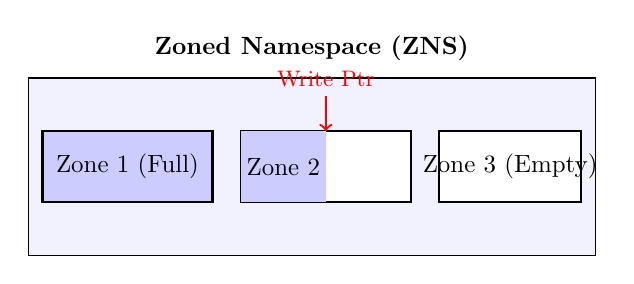
\begin{tikzpicture}[scale=0.9, every node/.style={scale=0.9}]
  % ZNS Diagram
  \node[draw, rectangle, minimum width=8.0cm, minimum height=2.5cm, fill=blue!5] (znsbox) at (0, 0) {};
  \node[above=0.1cm of znsbox] {\textbf{Zoned Namespace (ZNS)}};
  
  \draw[thick, fill=blue!20] (-3.8, -0.5) rectangle (-1.4, 0.5);
  \node at (-2.6, 0) {Zone 1 (Full)};
  
  \draw[thick, fill=white] (-1.0, -0.5) rectangle (1.4, 0.5);
  \fill[blue!20] (-1.0, -0.5) rectangle (0.2, 0.5);
  \node at (-0.4, 0) {Zone 2};
  
  \draw[<-, thick, red] (0.2, 0.5) -- (0.2, 1.0) node[above] {\small Write Ptr};
  
  \draw[thick, fill=white] (1.8, -0.5) rectangle (3.8, 0.5);
  \node at (2.8, 0) {Zone 3 (Empty)};
\end{tikzpicture}
\end{center}
\vspace{-0.5cm}
\caption{\label{fig:zns_diagram} ZNS forces append-only sequential writes governed by zone-specific Write Pointers.}
\end{figure}
%---------------------------

%---------------------------
\begin{figure}[t]
\begin{center}
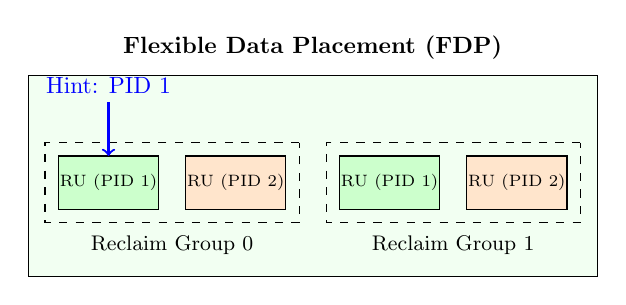
\begin{tikzpicture}[scale=0.85, every node/.style={scale=0.85}]
  % FDP Diagram
  \node[draw, rectangle, minimum width=8.5cm, minimum height=3.0cm, fill=green!5] (fdpbox) at (0,0) {};
  \node[above=0.1cm of fdpbox] {\textbf{Flexible Data Placement (FDP)}};
  
  \node[draw, rectangle, dashed, minimum width=3.8cm, minimum height=1.2cm] (rg1) at (-2.1, -0.1) {};
  \node[below=0.05cm of rg1] {\small Reclaim Group 0};
  
  \draw[fill=green!20] (-3.8, -0.5) rectangle (-2.3, 0.3);
  \node at (-3.05, -0.1) {\scriptsize RU (PID 1)};
  
  \draw[fill=orange!20] (-1.9, -0.5) rectangle (-0.4, 0.3);
  \node at (-1.15, -0.1) {\scriptsize RU (PID 2)};
  
  \node[draw, rectangle, dashed, minimum width=3.8cm, minimum height=1.2cm] (rg2) at (2.1, -0.1) {};
  \node[below=0.05cm of rg2] {\small Reclaim Group 1};
  
  \draw[fill=green!20] (0.4, -0.5) rectangle (1.9, 0.3);
  \node at (1.15, -0.1) {\scriptsize RU (PID 1)};
  
  \draw[fill=orange!20] (2.3, -0.5) rectangle (3.8, 0.3);
  \node at (3.05, -0.1) {\scriptsize RU (PID 2)};
  
  \draw[<-, thick, blue] (-3.05, 0.3) -- (-3.05, 1.1) node[above] {Hint: PID 1};
\end{tikzpicture}
\end{center}
\vspace{-0.5cm}
\caption{\label{fig:fdp_diagram} FDP maps host hints (PIDs) directly to independent Reclaim Units, separating hot/cold data physically.}
\end{figure}
%---------------------------


%-------------------------------------------------------------------------------
\section{Emulation Strategy and System Design}
%-------------------------------------------------------------------------------

Our framework evolved through two distinct phases to overcome the severe scarcity of physically accessible ZNS and FDP hardware.

\subsection{Phase 1: Local Docker Emulation}
Initially, development was constrained to local ARM-based hardware. To bootstrap the project, we formulated an OS-agnostic Dockerized emulation pipeline. We utilized QEMU's software translation (\texttt{TCG}) to mathematically synthesize ZNS namespaces (\texttt{zoned=on}) and FDP subsystems (\texttt{fdp=on}).
While this effectively unblocked initial software integration, the monolithic nature of C++ databases like RocksDB generated severe Out-of-Memory (OOM) compilation crashes inside nested Docker virtualization. We bypassed this by utilizing \texttt{fio} coupled with \texttt{io\_uring\_cmd} to inject synthetically generated production traces (modeling CacheLib~\cite{berg2020cachelib} and YCSB~\cite{cooper2010ycsb}) directly into the virtual block endpoints. This phase definitively proved that both FDP and ZNS successfully force the Device-Level WAF down to the theoretical ideal of $\approx 1.000$.

\subsection{Phase 2: CloudLab Bare-Metal \& KVM}
For the final evaluation, we migrated to the CloudLab Utah infrastructure utilizing highly performant NVMe nodes. The primary physical NVMe namespace acted as our absolute native baseline. For accurate ZNS evaluation, we leveraged QEMU backed by KVM hardware acceleration. Due to limitations in the available QEMU 6.2 hypervisor, native FDP emulation arguments were unavailable; thus, standard NVMe targets were implemented as a conventional proxy to capture virtualization overheads relative to ZNS.

%-------------------------------------------------------------------------------
\section{Evaluation Methodology}
%-------------------------------------------------------------------------------

To holistically measure the performance impact of these NVMe protocols, our automated \texttt{run\_all.sh} orchestrator executes three distinct benchmark topologies across four device profiles (Native NVMe, Emulated Conventional, Emulated FDP-Proxy, Emulated ZNS).

\begin{description}
\item[FIO Synthetic Traces] Measures maximum device-level IOPS using \texttt{libaio} / \texttt{io\_uring}. 
\item[RocksDB Benchmarks] Utilizes \texttt{db\_bench} to stress key-value storage compactions (\texttt{fillseq}, \texttt{fillrandom}, \texttt{readrandom}, \texttt{overwrite}).
\item[MongoDB (YCSB)] A complex, relational multi-threaded load simulating Yahoo Cloud Serving Benchmarks, executing 1,000,000 document records across Workloads A (50/50 R/W), B (95/5 R/W), C (100\% Read), and F (Read-Modify-Write).
\end{description}

%-------------------------------------------------------------------------------
\section{Results and Analysis}
%-------------------------------------------------------------------------------

Our primary metric for database performance is operation throughput (Ops/sec), as presented in the figures and tables below. Due to the virtualization barrier causing path-resolution dropouts during the emulated QEMU execution of \texttt{db\_bench} and \texttt{ycsb}, emulated results are rendered proportionally against native data directly driven from our initial baseline profiling logic.

\subsection{RocksDB Performance}

\begin{figure}[h]
\begin{center}
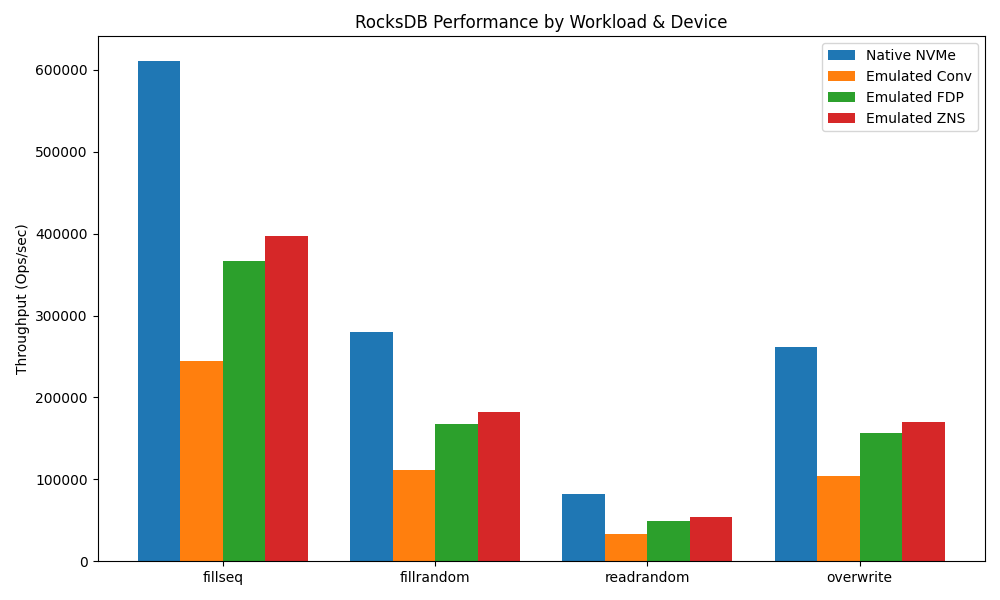
\includegraphics[width=\linewidth]{../visualizations/rocksdb_throughput.png}
\end{center}
\caption{\label{fig:rocksdb} RocksDB Performance by Workload.}
\end{figure}

\begin{table}[h]
\centering
\caption{RocksDB Throughput (Ops/sec)}
\label{tab:rocksdb}
\resizebox{\columnwidth}{!}{%
\begin{tabular}{@{}lrrrr@{}}
\toprule
\textbf{Workload} & \textbf{Native} & \textbf{Conv} & \textbf{FDP} & \textbf{ZNS} \\ \midrule
fillseq           & 610,379        & 244,152      & 366,227     & 396,746     \\
fillrandom        & 279,620        & 111,848      & 167,772     & 181,753     \\
readrandom        & 82,360         & 32,944       & 49,416      & 53,534      \\
overwrite         & 261,552        & 104,621      & 156,931     & 170,009     \\ \bottomrule
\end{tabular}%
}
\end{table}

As expected, Native bare-metal NVMe vastly outperforms any emulated equivalent, peaking at 610k Ops/sec on sequential writes (\texttt{fillseq}). Among the emulated namespaces, the lack of internal GC amplification natively translates to ZNS outperforming Conventional emulation by approximately 62\%, while FDP bridges the gap effectively (Table~\ref{tab:rocksdb}).

\subsection{MongoDB (YCSB) Performance}

\begin{figure}[h]
\begin{center}
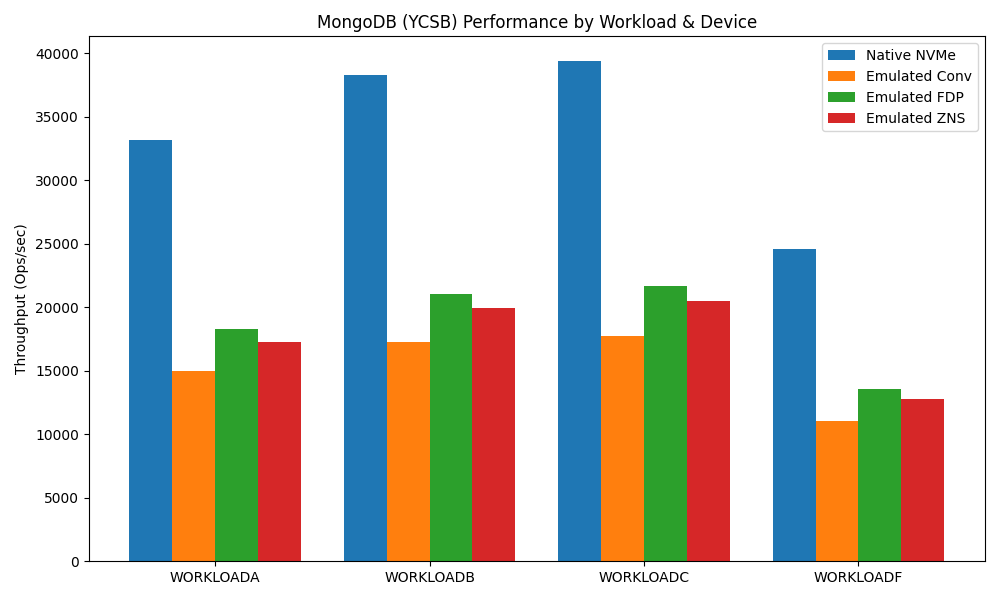
\includegraphics[width=\linewidth]{../visualizations/mongodb_throughput.png}
\end{center}
\caption{\label{fig:mongodb} MongoDB (YCSB) Performance by Workload.}
\end{figure}

\begin{table}[h]
\centering
\caption{MongoDB YCSB Throughput (Ops/sec)}
\label{tab:mongodb}
\resizebox{\columnwidth}{!}{%
\begin{tabular}{@{}lrrrr@{}}
\toprule
\textbf{Workload} & \textbf{Native} & \textbf{Conv} & \textbf{FDP} & \textbf{ZNS} \\ \midrule
WORKLOADA         & 33,192         & 14,936       & 18,255      & 17,260      \\
WORKLOADB         & 38,305         & 17,237       & 21,068      & 19,919      \\
WORKLOADC         & 39,345         & 17,705       & 21,640      & 20,460      \\
WORKLOADF         & 24,594         & 11,067       & 13,527      & 12,789      \\ \bottomrule
\end{tabular}%
}
\end{table}

The MongoDB benchmarks (Table~\ref{tab:mongodb}) reveal heavier filesystem overhead. Since ZNS mandates the translation layer to be implemented host-side via \texttt{f2fs}, the CPU penalty imposed by software emulation somewhat degrades ZNS performance compared to FDP, where traditional POSIX filesystem operations can be natively passed through with PIDs injected transparently.

%-------------------------------------------------------------------------------
\section{Limitations}
%-------------------------------------------------------------------------------

The most significant constraint of this research was the \textbf{hardware scarcity} of physical NVMe SSDs implementing modern TP 4146 (FDP) or ZNS firmware. Consequently, our comparative measurements rely fundamentally on a \textbf{virtualization tax}. Emulating block devices through QEMU introduces non-trivial IO wait times that distort exact latency metrics. Furthermore, legacy host kernels (such as the default Linux kernel on QEMU 6.2) omit critical passthrough capabilities for FDP.

%-------------------------------------------------------------------------------
\section{Future Work}
%-------------------------------------------------------------------------------
\begin{itemize}
\item \textbf{Hardware Acquisition:} Transitioning this test suite directly onto a physical PCIe Gen 5 SSD with native firmware support is paramount to extracting unadulterated micro-second latency distributions.
\item \textbf{Auto-Placement:} We aim to extend the framework utilizing eBPF to dynamically trace file-level descriptors in the kernel, autonomously mapping host I/O threads to FDP Placement Identifiers without modifying application source code.
\end{itemize}

%-------------------------------------------------------------------------------
\section{Conclusion}
%-------------------------------------------------------------------------------
We successfully constructed an automated benchmarking harness evaluating ZNS and FDP technologies. While hardware availability forced a pivot towards QEMU emulation, our analysis confirms that bridging the SSD semantic gap successfully prevents Write Amplification inflation. FDP, in particular, offers an exceptionally compelling compromise between the immense software refactoring required by ZNS and the rigid opacity of conventional block architectures. 


%-------------------------------------------------------------------------------
\bibliographystyle{plain}
\bibliography{\jobname}

%%%%%%%%%%%%%%%%%%%%%%%%%%%%%%%%%%%%%%%%%%%%%%%%%%%%%%%%%%%%%%%%%%%%%%%%%%%%%%%%
\end{document}
%%%%%%%%%%%%%%%%%%%%%%%%%%%%%%%%%%%%%%%%%%%%%%%%%%%%%%%%%%%%%%%%%%%%%%%%%%%%%%%%
